\documentclass[border=10pt]{standalone}

\usepackage{tikz}
\usepackage{tikzsymbols}
\usetikzlibrary{calc,patterns,shapes.geometric}

\def\centerarc[#1](#2)(#3:#4:#5){\draw[#1] ($(#2)+({#5*cos(#3)},{#5*sin(#3)})$) arc (#3:#4:#5);}

\begin{document}
	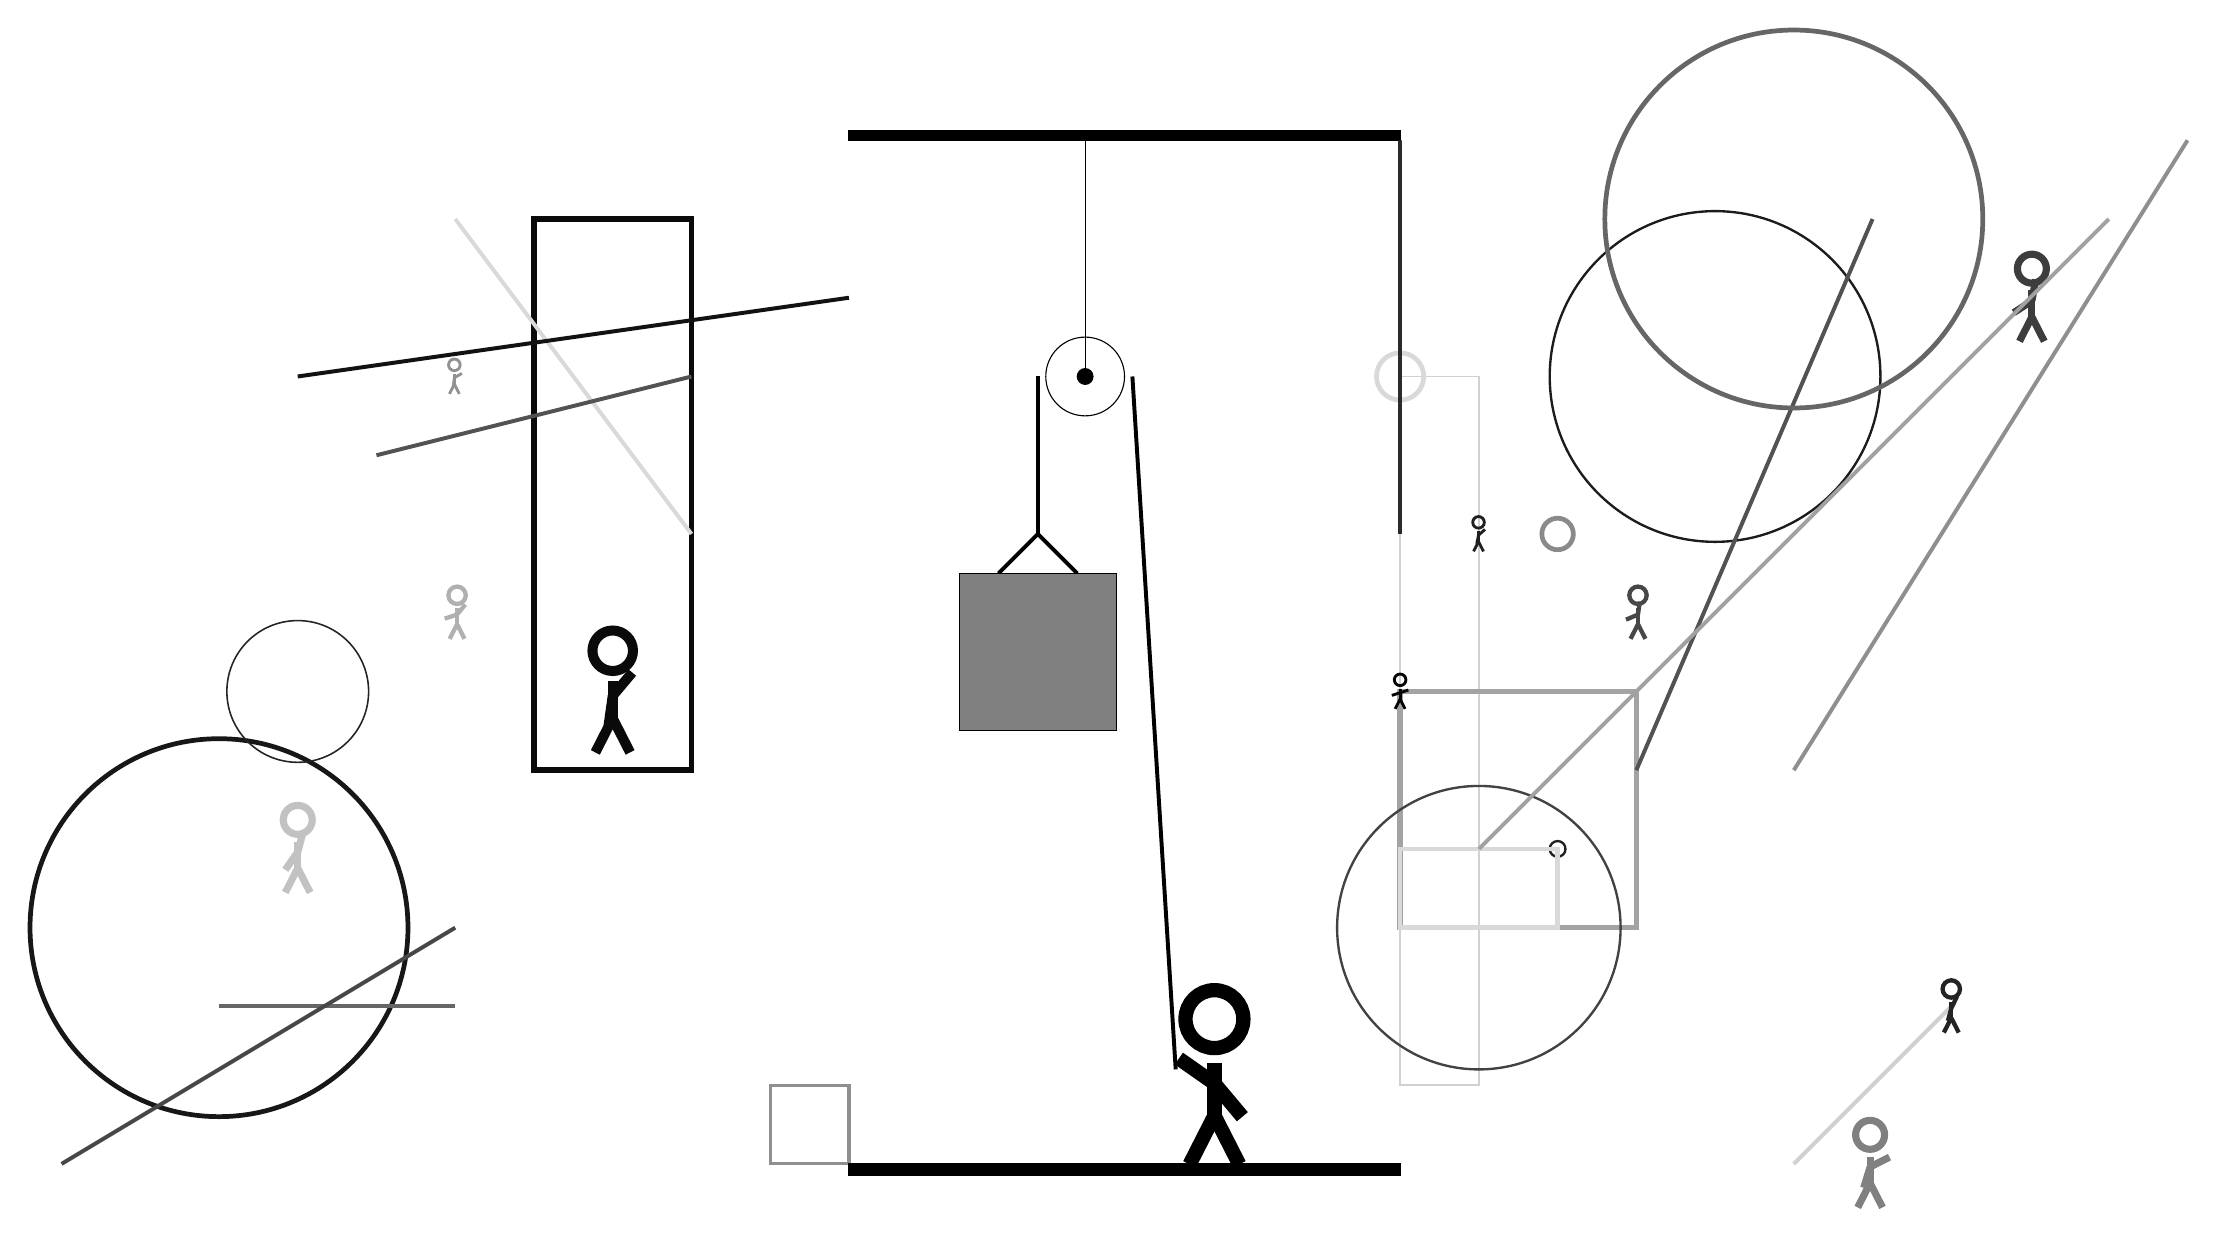
\begin{tikzpicture}
		%%%%% START %%%%%
		
		\draw[fill=black] (-2, 10) rectangle (5, 10.125);
		
		\draw (1, 7) circle (0.5);
		\draw[fill=black] (1, 7) circle (0.1);
		\draw (1, 10) -- (1, 7);
		
		\draw[line width=0.5mm] (-0.1, 4.5) -- (0.4, 5.0) -- (0.9, 4.5);
		\draw[fill=black!50] (-0.6, 4.5) rectangle (1.4, 2.5);
		
		\draw[line width=0.5mm] (0.4, 7) -- (0.4, 5.0);
		\centerarc[line width=0.5mm](1, 7)(0:180:0.6);
		\draw[line width=0.5mm](1.6, 7) -- (2.15, -1.8);
		
		\node[line width=0.6mm, color=black!72] at (8, 4) {\Strichmaxerl[3][23][82]};
		
		\node[line width=0.6mm, color=black!31] at (-7, 4) {\Strichmaxerl[3][18][51]};
		\draw[line width=0.2mm, color=black!18] (6, 7) rectangle (5, -2);
		\draw [line width=0.3mm, color=black!87](7, 1) circle (0.1);
		\node[line width=0.5mm, color=black!88] at (6, 5) {\Strichmaxerl[2][78][42]};
		
		\draw[line width=0.7mm, color=black!36] (5, 3) rectangle (8, 0);
		\draw[line width=0.7mm, color=black!96] (-4, 2) rectangle (-6, 9);
		\draw[line width=0.5mm, color=black!18](10, -3) -- (12, -1);
		\node[line width=0.5mm, color=black!86] at (12, -1) {\Strichmaxerl[3][75][64]};
		\draw [line width=0.6mm, color=black!46](7, 5) circle (0.2);
		\draw[line width=0.5mm, color=black!44](10, 2) -- (15, 10);
		\node[line width=0.4mm, color=black!43] at (-7, 7) {\Strichmaxerl[2][83][30]};
		\draw [line width=0.6mm, color=black!15](5, 7) circle (0.3);
		
		\node[line width=0.4mm, color=black!50] at (11, -3) {\Strichmaxerl[5][73][27]};
		\draw[line width=0.4mm, color=black!44] (-2, -3) rectangle (-3, -2);
		\draw [line width=0.6mm, color=black!91](-10, 0) circle (2.4);
		
		\node[line width=0.5mm, color=black!24] at (-9, 1) {\Strichmaxerl[5][55][75]};
		\draw[line width=0.5mm, color=black!15](-7, 9) -- (-4, 5);
		\draw [line width=0.3mm, color=black!89](9, 7) circle (2.1);
		\draw [line width=0.3mm, color=black!74](6, 0) circle (1.8);
		\draw[line width=0.5mm, color=black!68](8, 2) -- (11, 9);
		\draw[line width=0.5mm, color=black!83] (5, 10) rectangle (5, 5);
		\draw[line width=0.6mm, color=black!15] (5, 1) rectangle (7, 0);
		\node[line width=0.2mm, color=black!98] at (5, 3) {\Strichmaxerl[2][18][18]};
		\node[line width=0.4mm, color=black!96] at (-5, 3) {\Strichmaxerl[7][82][50]};
		
		\draw [line width=0.2mm, color=black!86](-9, 3) circle (0.9);
		
		\draw[line width=0.5mm, color=black!68](-4, 7) -- (-8, 6);
		\draw [line width=0.6mm, color=black!60](10, 9) circle (2.4);
		\draw[line width=0.5mm, color=black!93](-2, 8) -- (-9, 7);
		
		\draw[line width=0.5mm, color=black!60](-7, -1) -- (-10, -1);
		\node[line width=0.2mm, color=black!76] at (13, 8) {\Strichmaxerl[5][33][80]};
		\draw[line width=0.5mm, color=black!72](-7, 0) -- (-12, -3);
		\draw[line width=0.5mm, color=black!37](6, 1) -- (14, 9);
		
		\node at (2.6, -1.9) {\Strichmaxerl[10][-35][-50]};
		
		\draw[fill=black] (-2, -3) rectangle (5, -3.15);
		
		%%%%% END %%%%%
	\end{tikzpicture}
\end{document}